\section{3D Geometry and Camera Calibration}
\subsection{Basics}
\b{Pinhole Camera:} The most popular projection model, even though it neglects the effect of lenses. In this model, a 3D point \f{X = \top{(X,Y,Z)}} is projected onto a point in the image plain via:
\cf{x = f\frac{X}{Z}\quad,\quad y=f\frac{Y}{Z}}
This projection is nonlinear due to the division by \f{Z}, meaning the height in the image plane is not linear to the real height \f{Z}.\\
To avoid this nonlinearity in calculations, we can work in so-called homogenous coordinates by adding a 1 to the end of the coordinate vector:
\cf{
    (x,y)\in\mathbb{R}^2\quad\to\quad(x,y,1)\in\mathbb{P}^2
}
To get back to Euclidian space we simply have to divide by the third coordinate.\\

Using homogenous coordinates, the projection from above becomes linear (only when recalculating the Euclidian coordinates we have to divide):
\cf{
    \begin{pmatrix}
        x' \\
        y' \\
        z' 
    \end{pmatrix} =  
    \begin{pmatrix}
        f & 0 & 0 & 0 \\
        0 & f & 0 & 0 \\
        0 & 0 & 1 & 0 
    \end{pmatrix} \begin{pmatrix}
        X \\
        Y \\
        Z \\
        1 
        \end{pmatrix}
}
\cf{
    x=\frac{x'}{z'}\quad,\quad y=\frac{y'}{z'}
}
The linear operator \f{P} is called \b{projection matrix} with \f{x=PX}. So far the matrix has many zero entries. In general, all 12 entries are different from zero describing a general projective camera. However, the matrix has only 11 degrees of freedom because scaling does not change the resulting 2D point (in Euclidean coordinates).\\
The task to determine the entries of the projection matrix is called \b{camera calibration}. Knowing the projection matrices of the involved cameras is required for 3D point reconstruction from 2D point correspondences. \\

The projection matrix can be factorized into two parts \f{P=KM}, where:
\cf{K=\begin{pmatrix}
    \alpha_x & s & x_0 \\
    0 & \alpha_y & y_0 \\
    0 & 0 & 1 
    \end{pmatrix}}
is the \b{camera calibration matrix} containing the camera's internal parameters. The second part, \f{M=(R|t)}, is the pose of the camera relative to a world coordinate system. \f{M} consists of a rotation matrix \f{R} and a translation vector \f{t}, each having 3 degrees of freedom. These are the external parameters.\\

\b{Note:} \f{P} must have rank 3 to project to a plane.\\

\b{Meaning of the parameters of K:}
\begin{itemize}
    \item \f{\alpha_x}: focal length times pixel width in x-direction
    \item \f{\alpha_y}: focal length times pixel width in y-direction
    \item \f{x_0,y_0}: origin in the image plane (principal point)
    \item \f{s=\alpha_x\cos\phi}: skew parameter (almost always 0)
\end{itemize}
\newpage
\b{Note:} if \f{\alpha_x=\alpha_y} then the pixels are square and the number of free parameters decreases. The other parameters vary from camera to camera and must be determined by a calibration procedure. The focal length may even change while recording a video, e.g. because of autofocus.\\

\b{Affine projection / camera model:}
The \b{affine projection} is an approximation of the perspective projection that leads to linear mappings also in Euclidean coordinates. The \b{affine camera model} only has 8 free parameters:
\cf{
    P = \begin{pmatrix}
        m_{11} & m_{12} & m_{13} & t_1 \\
        m_{21} & m_{22} & m_{23} & t_2 \\
        0 & 0 & 0 & 1 
        \end{pmatrix}
}
\b{Note:} This camera model is (only) a good approximation if objects are far from the camera and have a small variation in depth.


\subsection{Camera Calibration}
Camera calibration denotes the process that estimates the camera parameters from suitable images. \b{Full calibration} yields the projection matrices of all involved cameras in a common world coordinate system. For this we need information about the true size of the observed object and its pose in the world coordinate system. Sometimes this is not available, e.g., in structure from motion. In this case the calibration procedure shall determine the camera's internal parameters.\\

\b{Full Camera Calibration from 2D-3D Correspondences:\\[0.5em]}
The classical procedure is based on a \b{calibration object} with known 3D points (e.g. black squares image). Observation of these points in the image yields 2D-3D correspondences.\\
In the example of the image with the black squares, the 2D point correspondences could be found by a corner detector. This works by applying an edge detector, then fitting lines to the edges (Hough transform) and finding the crossings of the lines.\\
From the retrieved point pairs \f{x_i,X_i} we can estimate the camera parameters. Each point correspondence has the constraint:
\cf{x_i\times PX_i = 0}
Since we are in homogenous coordinates, two points are equivalent if their vectors have the same direction, which is expressed by the cross product.\\

\begin{figure}[h!]
    \centering
    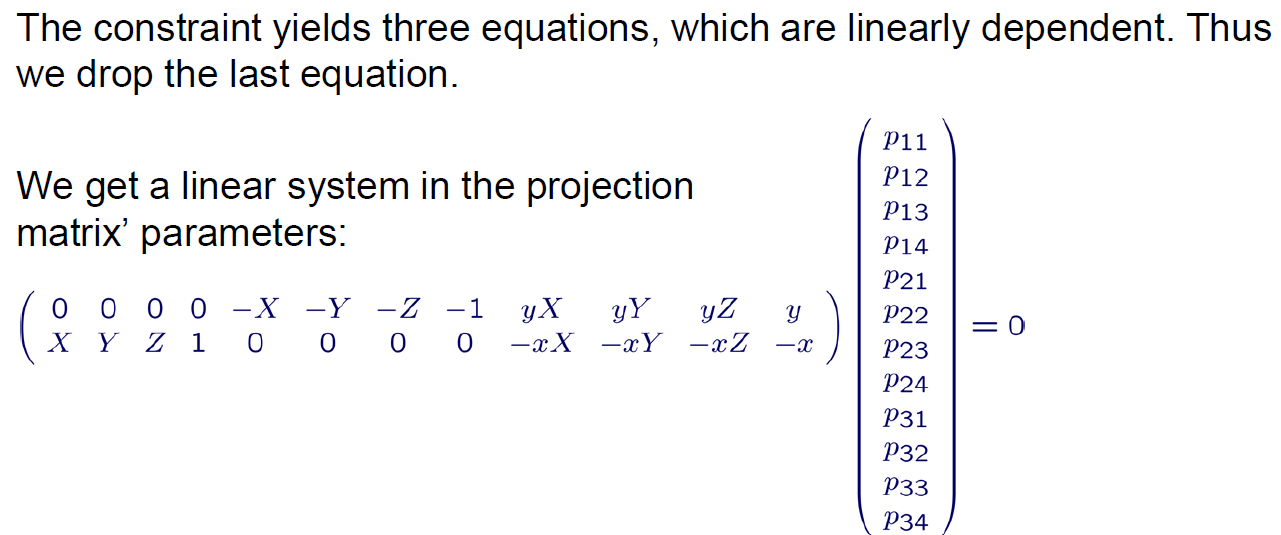
\includegraphics[width=0.6\textwidth]{cali.png}
\end{figure}

For each point correspondence we get such a system and by stacking the equations we get a system with \f{2N\times 12} \b{system matrix} \f{A}. We need at least 6 point correspondences. All we have to do is solve (minimize) the over-determined system \f{Ap=0} while avoiding the trivial solution \f{p=0}.\\
Note that we have 12 parameters but only 11 degrees of freedom. The best way is to introduce the constraint \f{||p||=1}. Then we end up with the minimization problem of \f{\frac{||Ap||}{||p||}}. This can be achieved by SVD (quite complex to compute). The solution is just the singular vector corresponding to the smallest singular value (not \it{eigen}, since A is not quadratic).
\newpage
\b{Normalization:\\[0.5em]}
The accuracy of the calibration matrix depends on the accuracy of the extracted corner points in the image. For accurate estimates it is important that the errors are treated homogeneously. This can be achieved by normalizing the 3D points as well as the 2D points such that their centroids are at 0 and the average distance of points to the centroid is \f{\sqrt{3}} and \f{\sqrt{2}} respectively.\\
The transformations to do so (shift and scaling) are expressed by matrices \f{U} and \f{T}. We then estimate the projection matrix \f{\tilde{P}} with the transformed points and retrieve \f{P} by \f{P=T^{-1}\tilde{P}U}.\\

\b{Note:} Up to this point the procedure only works if the calibration object (the 3D points) is \b{coplanar}. This requires a calibration object of at least two planes (precise measurement rather difficult).\\

\b{Note:} An alternative calibration method would be from multiple views of the same \it{planar} calibration object. Except for multi-camera setups this is much more convenient.

\subsection{General Projection to Homography}
In general, the projection is described as follows:
\cf{
    \begin{pmatrix}
    x \\
    y \\
    1 
\end{pmatrix} = K\cdot
\begin{pmatrix}
    r_1 & r_2 & r_3 & t
\end{pmatrix}
\begin{pmatrix}
    X \\
    Y \\
    Z \\
    1 
    \end{pmatrix}}
But now that all points lie in a plane, we can, without loss of generality, choose the world coordinate system such that this plane is \f{Z=0}:
\cf{
\begin{pmatrix}
    x \\
    y \\
    1 
\end{pmatrix} = K\cdot
\begin{pmatrix}
    r_1 & r_2 & r_3 & t
\end{pmatrix}
\begin{pmatrix}
    X \\
    Y \\
    0 \\
    1 
\end{pmatrix} = K\cdot
\begin{pmatrix}
        r_1 & r_2 & t
    \end{pmatrix}
\begin{pmatrix}
        X \\
        Y \\
        1 
\end{pmatrix}
}
The projection is a plane to plane mapping involving only 2D coordinates. Such a mapping is described by a homography (\f{x' = Hx}), which can be estimated by 2D point correspondences.\\

Homography estimation works the same way as estimation of the projection matrix discussed before. \f{H} is even a projection in a simplified setting (all points lying in a plane). With the constraint that all corresponding points must have the same direction
(\f{x'\times Hx = 0}), 
we can obtain three linear dependent equations from each point correspondence (we only keep two):
\cf{
    \begin{pmatrix}
        0&0&0-x&-y&-1&y'x&y'y&y'\\
        x&y&1&0&0&0&-x'x&-x'y&-x'
    \end{pmatrix}h=0
} 
Considering \f{n} correspondences we get a linear system \f{Ah=0} with \f{A\in\mathbb{R}^{2n\times 9}}, subject to \f{||h||=1}. The solution can again be obtained by SVD. To treat errors in the correspondences homogeneously the points should again be normalized. This can be done by applying a normalizing transformation \f{T} to all points \f{x_i} such that the centroid is in the origin and the average distance to the origin is \f{\sqrt{2}}.\\

\b{Homography decomposition:\\[0.5em]}
The estimated homographycontains the internal and external camera parameters:
\cf{H=K\cdot(r_1\ r_2\ t) \qquad (h_1\ h_2\ h_3) = \lambda K\cdot(r_1\ r_2\ t)}
From this, we can derive two constraints for decomposition: (1) \f{r_1} and \f{r_2} must be orthogonal, (2) the rotation vector itself should be 1.
\newpage

Since we have two equations (restraints) for 5 unknowns, either three of the internal camera parameters need to be known or we need additional constrains from further homographies! These homographies are obtained by moving the camera (or the plane). The motion must comprise a rotation and the internal parameters must not change. At least 3 views are needed to estimate all 5 parameters. Once the internal parameters are known, the external parameters for each view can be estimated.\\

\b{Left out: Mathematical decomposition process}\\

\b{Note:} Due to estimation errors, the rotation matrix is usually not a proper rotation matrix with \f{R^\top R=1}. This can be enforced by applying an SVD \f{R=UDV^\top}.

\subsection{Radial Distortion}
With the pinhole camera model the projection was a linear operation in homogenous coordinates. However, the pinhole camera neglects the effect of lenses, which have a nonlinear effect on the projection (can not be described by projection matrix). This effect becomes increasingly relevant for decreasing focal length (e.g. fisheye effect). The distortion can be modeled as:
\cf{
    \begin{pmatrix}
        x\\
        y
    \end{pmatrix} = L(r)
    \begin{pmatrix}
        \tilde{x}\\
        \tilde{y}
    \end{pmatrix}
}
where \f{L(r)} is a function that depends only on the distance of a point to the center of distortion (usually the principal point \f{(x_0,y_0)} of the camera). \f{L(r)} can be modeled as:
\cf{
    L(r) = 1+\kappa_1r+\kappa_2r^2+\kappa_3r^3+...
}
The coefficients can be estimated from the correspondences by minimizing a cost function that penalizes the deviation from the linear mapping in the calibration procedure:
\begin{itemize}
    \item Calculate ideal distortion free projected points \f{(\tilde{x}, \tilde{y})} with \f{P}
    \item Calculate distance \f{r=\sqrt{(\tilde{x}-x_0)^2+(\tilde{y}-y_0)^2}} from principal point to projected points
    \item Observe/measure the actual image point (not the projected one)
    \item Calculate coefficients of \f{L(r)} to compensate displacement of points
\end{itemize}

\newpage